\documentclass[border=10pt]{standalone}
\usepackage[utf8]{inputenc}
\usepackage{tikz}
\usetikzlibrary{arrows,decorations.pathmorphing,backgrounds,fit,positioning,shapes.symbols,chains,shapes.geometric,shapes.arrows,calc}

\begin{document}
  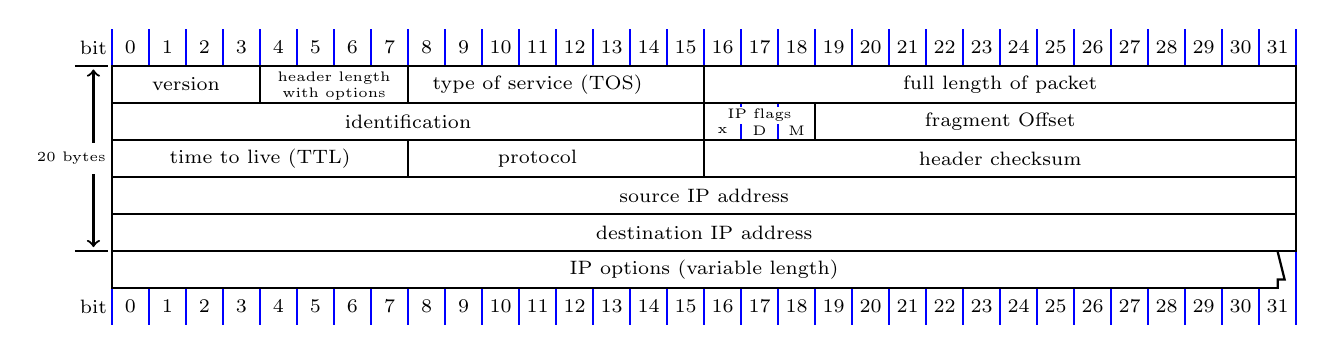
\begin{tikzpicture}[scale=0.47]
	\foreach \x in {0,...,31}
		\node at (\x+0.5,20.5) {\scriptsize \x};
	\foreach \x in {0,...,31}
		\node at (\x+0.5,13.5) {\scriptsize \x};
	\foreach \x in {0,...,32}
		\draw[thick, blue] (\x,13) -- (\x,21);
	\node[thick] (bit1) at (-0.5,20.5) {\scriptsize bit};
	\node[thick] (bit2) at (-0.5,13.5) {\scriptsize bit};
	\draw [<->, thick] (-0.5, 19.9) -- (-0.5,15.1);
	\draw [thick] (-1, 20) -- (-0.1,20);
	\draw [thick] (-1, 15) -- (-0.1,15);
	\node[fill=white] at (-1.1,17.5) {\tiny 20 bytes};
	\filldraw[thick,draw=black, fill=white] (0,20) rectangle (4,19); \node (mode) at (2,19.5) {\scriptsize version};
	\filldraw[thick,draw=black, fill=white] (4,20) rectangle (8,19); \node (mode) at (6,19.68) {\tiny header length};\node (mode) at (6,19.25) {\tiny with options};
	\draw[thick, draw=black, fill=white] (8,20) rectangle (16,19); \node (stratum) at (11.5,19.5) {\scriptsize type of service (TOS)};
	\draw[thick, draw=black, fill=white] (16,20) rectangle (32,19); \node (li) at (24,19.5) {\scriptsize full length of packet};
	\filldraw[thick,draw=black, fill=white] (0,19) rectangle (16,18); \node (mode) at (8,18.5) {\scriptsize identification};
	\draw[thick, draw=black] (16,19) rectangle (19,18); \filldraw[white] (16.5,18.43) rectangle (19,18.88); \node [](li) at (17.5,18.67) {\tiny IP flags}; \node at (16.5,18.25) {\tiny x};\node at (17.5,18.25) {\tiny D};\node at (18.5,18.25) {\tiny M};
	\draw[thick, draw=black, fill=white] (19,19) rectangle (32,18); \node (li) at (24,18.5) {\scriptsize fragment Offset};
	\filldraw[thick,draw=black, fill=white] (0,18) rectangle (8,17); \node (mode) at (4,17.5) {\scriptsize time to live (TTL)};
	\draw[thick, draw=black, fill=white] (8,18) rectangle (16,17); \node (stratum) at (11.5,17.5) {\scriptsize protocol};
	\draw[thick, draw=black, fill=white] (16,18) rectangle (32,17); \node (li) at (24,17.5) {\scriptsize header checksum};
	\filldraw[thick,draw=black, fill=white] (0,17) rectangle (32,16); \node (mode) at (16,16.5) {\scriptsize source IP address};
	\filldraw[thick,draw=black, fill=white] (0,16) rectangle (32,15); \node (mode) at (16,15.5) {\scriptsize destination IP address};
	\draw[thick,draw=black, fill=white] (0,15) rectangle (31.5,14);
	\draw[fill=white, draw=white] (31.4,14.96) rectangle (31.6,14.05);
	\draw[thick]  (31.5,14.97)  decorate [decoration=saw] { -- (31.5,14.02)};
	\node (mode) at (16,14.5) {\scriptsize IP options (variable length)};
	\end{tikzpicture}
\end{document}
